% Lab 1 report
% Build:  latexmk -pdf main.tex     (inside report/)
\documentclass[11pt,a4paper]{article}
\usepackage[margin=2.4cm]{geometry}
\usepackage[utf8]{inputenc}
\usepackage[T1]{fontenc}
\usepackage{amsmath,amssymb,graphicx,booktabs,listings,caption,float}
\usepackage[hidelinks]{hyperref}
\captionsetup{font=small,labelfont=bf}
\lstset{basicstyle=\ttfamily\scriptsize,breaklines=true,frame=single,numbers=left,numberstyle=\tiny,language=Python,
  inputencoding=utf8,extendedchars=true,showstringspaces=false}
\setlength{\emergencystretch}{2em}
\newcommand{\codelisting}[2]{\IfFileExists{#1}{\lstinputlisting[caption={\texttt{#2}}]{#1}}{\par\noindent\textit{(#2 not found at build time)}\par}}
\newcommand{\kB}{k_{\mathrm B}}
\newcommand{\Om}{\Omega}

\title{Microstates and Macroscopic Thermodynamics of a Binary System\\[2pt]\large Statistical Physics --- Laboratory Practice 1}
\author{Marta Alonso Pérez (100549892/100549892) \and Teo Biaggini Cervantes (100542175/100542175) \and Eduardo Martín Millán (100550999/100550999) \and Saulo Muriel Carmona (100551014/100551014)\\[4pt]
Department of Physics, Universidad Carlos III de Madrid}
\date{4 November 2026}

\begin{document}
\maketitle

\begin{abstract}
A system of $N$ independent unbiased coins is used as an exact model of a two-state assembly. All
$2^N$ microstates are enumerated with a bitwise generator (memory $O(N)$, one counter per macrostate); the time doubles with every
added coin, which limits full enumeration to $N\approx31$ in five minutes, while storing every state
exhausted the RAM at $N=28$ ($N=27$ completed in 104~s). The multiplicity $\Om(N,k)$ is computed in log-space with the
log-gamma function, which removes the double-precision overflow that stops direct evaluation at $N\approx10^3$.
For the team size $N=138$ the most probable macrostate has $P_{69}=0.068$ and $92.7\%$ of the probability lies within
$\pm10$ heads of it; the ordered macrostate with 20 heads has $38.2\,\kB$ less entropy, and reaching 8 heads by random tossing
takes $\sim4\times10^{21}$ years. For $N\sim10^{23}$ the distribution is a Gaussian of relative width
$3.2\times10^{-12}$, so the Second Law becomes deterministic. Code and tests:
\url{https://github.com/100542175/LAB-1-STATISTICAL-PHYSICS}.
\end{abstract}

\section{Introduction}
A \emph{microstate} is the configuration of all $N$ coins (e.g.\ HHTHT); a \emph{macrostate} is fixed by the number
of heads $k$ and contains
\begin{equation}
  \Om(N,k)=\binom{N}{k}=\frac{N!}{k!\,(N-k)!},\qquad \sum_{k=0}^{N}\Om(N,k)=2^N
  \label{eq:omega}
\end{equation}
equiprobable microstates. The probability of a macrostate is $P_k=\Om(N,k)/2^N$ and its Boltzmann entropy is
$S=\kB\ln\Om$. We study the computational limits of enumerating microstates and of evaluating $\Om(N,k)$ (Part~1), the
probabilities, entropy changes and waiting times for a team-specific $N=100+M$ (Part~2), and the extrapolation to
$N\sim10^{23}$ (Sections~\ref{sec:thermo} and~\ref{sec:largeN}).

\section{Methodology}
The code is written in Python in a Conda environment (NumPy, SciPy, Matplotlib, pytest) and organised in modules
(\texttt{combinatorics}, \texttt{microstates}, \texttt{thermodynamics}, \texttt{plots}), with unit tests and a
\texttt{main.py} that reproduces every figure and number. Microstates are integers $s\in[0,2^N)$ (bit $i=1$: coin $i$ is heads),
generated with \texttt{yield} up to \texttt{1 << N}; the number of heads is the population count of $s$. Large multiplicities
are computed in log-space,
\begin{equation}
  \ln\Om(N,k)=\ln\Gamma(N+1)-\ln\Gamma(k+1)-\ln\Gamma(N-k+1),
  \label{eq:lngamma}
\end{equation}
and validated with \texttt{pytest} against exact integers (\texttt{math.comb}) for $N\le199$ and all $k$.
Probabilities and entropies are exact calculations, so their only uncertainty is floating-point rounding, quantified by this
comparison; timings are mean $\pm$ standard deviation of repeated runs. All quantities are dimensionless unless a unit is given.

\section{Part 1: computational analysis of microstates}
\subsection{Enumeration for $N=7$}
With $2^7=128$ microstates and $N+1=8$ macrostates, Table~\ref{tab:n7} lists the multiplicities obtained by
enumerating all states with the program; every microstate is listed in Appendix~\ref{app:n7}.
\begin{table}[H]
\centering\small
\begin{tabular}{@{}cccl@{}}
\toprule
heads $k$ & tails $7-k$ & $\Om(7,k)$ & example microstate \\ \midrule
7 & 0 & 1 & HHHHHHH \\ 6 & 1 & 7 & HHHHHHT \\ 5 & 2 & 21 & HHHHHTT \\ 4 & 3 & 35 & HHHHTTT \\
3 & 4 & 35 & HHHTTTT \\ 2 & 5 & 21 & HHTTTTT \\ 1 & 6 & 7 & HTTTTTT \\ 0 & 7 & 1 & TTTTTTT \\ \bottomrule
\end{tabular}
\caption{Macrostates of $N=7$ coins ($\Om$ dimensionless, exact integers, no uncertainty; sum $=128=2^7$).}
\label{tab:n7}
\end{table}

\subsection{Largest $N$ with full enumeration}
The number of microstates doubles with each added coin, $2^{N+1}/2^N=2$, so the cost is exponential in both time and memory.
\textbf{Storing every state} as a string needs $\propto N\,2^N$ bits; in CPython each string object costs $\sim N+40$ bytes plus an
8-byte list pointer, i.e.\ $\approx10$~GB at $N=27$ and $\approx21$~GB at $N=28$ (estimate). Measured with this approach, $N=27$
($2^{27}=134\,217\,728$ states) completed in 104.3~s, while $N=28$ stopped because the RAM was exhausted. The limit is therefore
\emph{memory}, not time.

\textbf{Generator.} Visiting the states with a generator and keeping only one counter per macrostate needs $O(N)$ memory (peak
$\approx0.7$~kB versus $0.65$~MB for storing all states at $N=14$), so the time becomes the limit. The measured time grows as $2^N$
(Fig.~\ref{fig:time}: $\approx0.5$~s at $N=22$), and extrapolating this scaling to the five-minute budget gives
$N_{\max}\approx31$ (extrapolated, not measured up to that value).
\begin{figure}[H]
\centering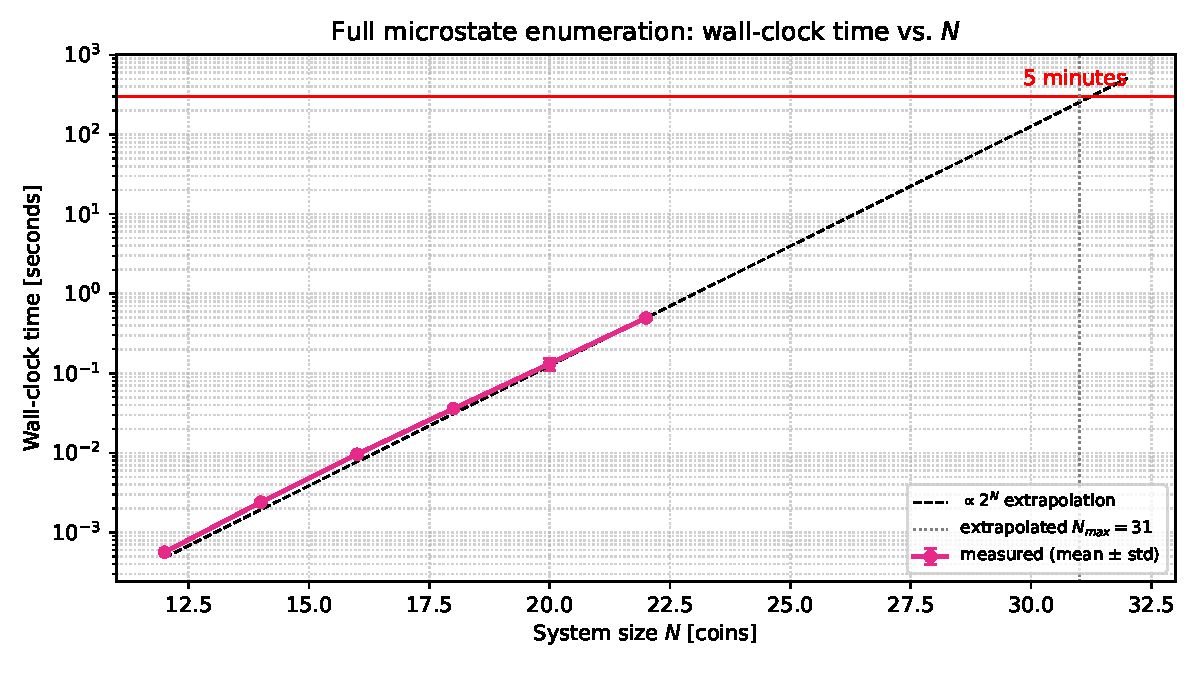
\includegraphics[width=0.62\textwidth]{figures/figure_timing}
\caption{Wall-clock time (s) of the full enumeration versus $N$ (mean $\pm$ std of repeated runs, log scale). Dashed: $\propto2^N$
extrapolation; red: five minutes; dotted: extrapolated $N_{\max}=31$.}
\label{fig:time}
\end{figure}

\subsection{Macrostate distributions for $N=20,50,80,100$}
Figure~\ref{fig:dist} shows $P_k=\Om(N,k)/2^N$ (left) and $\Om(N,k)$ on a logarithmic scale (right) for the four sizes.
All distributions are symmetric about $k=N/2$ (all $N$ are even) and peak there: $\Om(N,N/2)=1.85\times10^{5},\ 1.26\times10^{14},\
1.08\times10^{23},\ 1.01\times10^{29}$ and $P_{N/2}=0.176,\ 0.112,\ 0.089,\ 0.080$. For $N=100$, the total is $2^{100}=1.27\times10^{30}$.
Because $\Om$ differs by many orders of magnitude between sizes, on a linear axis only the largest curve would be visible; hence
the log scale and the normalised probability.
\begin{figure}[H]
\centering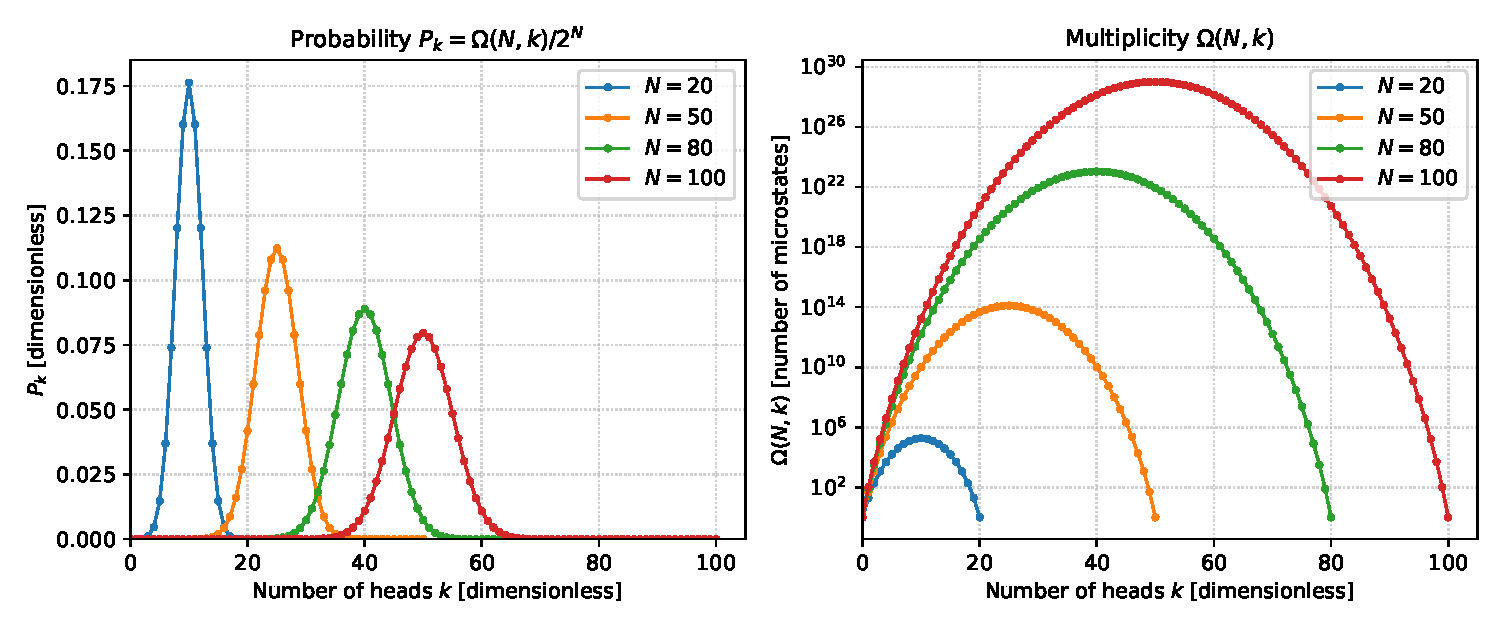
\includegraphics[width=0.95\textwidth]{figures/figure_distributions}
\caption{Left: probability $P_k$ versus number of heads $k$ (dimensionless). Right: multiplicity $\Om(N,k)$ (number of
microstates, log scale). Values are exact to $\sim10^{-13}$ relative.}
\label{fig:dist}
\end{figure}

\subsection{Largest $N$ for the distribution}
Computing the $N+1$ coefficients with the recurrence $\Om(N,0)=1$, $\Om(N,k+1)=\Om(N,k)(N-k)/(k+1)$ in exact integers
avoids generating $2^N$ states. Two tests (300~s limit each) gave different limits.
\emph{Calculation:} all coefficients were obtained up to $N=354\,419$, beyond which the RAM was exhausted, since each coefficient is an
integer of $\sim N$ bits and the total memory grows $\propto N^2$.
\emph{Plotting:} the largest size plotted without error was $N=1028$, because converting the integers to
double precision overflows above $\sim1.8\times10^{308}$ (the exact threshold for $\Om(N,N/2)$ is $N=1029$).
This limit is not fundamental: computing in log-space \eqref{eq:lngamma} avoids the overflow entirely, and the
accuracy then limits $N$ only through rounding ($|\sum_kP_k-1|=6\times10^{-13}$ at $N=10^3$ and $1\times10^{-8}$ at $N=10^7$,
with $\approx80$~MB per array at $N=10^7$). The practical maximum is therefore $N\sim10^7$ in double precision, limited by
memory and accuracy, versus $N=1028$ for direct integer-to-float conversion.

\subsection{Thermodynamic limit}
For $N$ fair coins $k$ is binomially distributed with $\mu=N/2$ and $\sigma=\sqrt N/2$. By Stirling's formula, with $x=k-N/2$ and
$|x|\ll N$,
\begin{equation}
  P_k\simeq\sqrt{\frac{2}{\pi N}}\,e^{-2x^2/N},\qquad
  \frac\sigma\mu=\frac1{\sqrt N},\qquad
  \ln\Om\left(N,\tfrac N2+x\right)\simeq N\ln2+\tfrac12\ln\frac2{\pi N}-\frac{2x^2}{N}.
  \label{eq:gauss}
\end{equation}
For $N=10^{23}$: $\mu=5\times10^{22}$, $\sigma=1.58\times10^{11}$ heads, and $\sigma/\mu=3.16\times10^{-12}$. The
absolute fluctuation is huge but the relative one is negligible: the distribution is a spike at $k/N=\tfrac12$ (a deviation
$k/N=\tfrac12+\delta$ has probability $\sim e^{-2N\delta^2}$), so the macroscopic state is sharply defined although each coin is random.
Since $S=\kB\ln\Om$ is largest at $k=N/2$, the equilibrium macrostate coincides with the maximum-entropy one, and
$\Delta S\propto N\kB$ between it and ordered states is macroscopic.

\section{Part 2: probabilities, entropy and thermodynamics}
The team size is $N=100+M$, where $M$ is the harmonic mean of the last two digits of the team members' NIAs (92, 75, 99 and 14):
\begin{equation}
M=\frac{n}{\sum_{i=1}^{n}\frac{1}{x_i}}=\frac{4}{\frac1{92}+\frac1{75}+\frac1{99}+\frac1{14}}=37.83\simeq38,\label{eq:M}
\end{equation}
with $n=4$ members and $x_i$ the last two NIA digits. Rounding to the nearest integer gives $M=38$ and $N=138<200$.
No digit is zero, so no replacement was needed in the harmonic mean. As $N$ is even, $N/2=69$ is an
integer. All quantities are computed in log-space with
$\ln\Om(N,k)=\ln\Gamma(N+1)-\ln\Gamma(k+1)-\ln\Gamma(N-k+1)$, which avoids overflow
($2^{138}=3.48\times10^{41}$, $\Om(138,69)=2.36\times10^{40}$). They are exact up to floating-point rounding, which is
the only source of uncertainty and is quantified by comparison with exact integer arithmetic
(\texttt{math.comb}).

\subsection{Probabilities}
Table~\ref{tab:prob} gives $P_k=\Om(N,k)/2^N$ for items a) and b), and the cumulative probability $\Delta P_{k_1k_2}=\sum_{k=k_1}^{k_2}P_k$ for items c) and d).
Since the distribution is symmetric under $k\to N-k$, a range of $N/2\pm20$ \emph{tails} (item d) is the same as $N/2\pm20$ heads.
\begin{table}[H]
\centering
\begin{tabular}{@{}cllr@{}}
\toprule
item & quantity & range & value \\ \midrule
a) & $P_{30}$ & $k=30$ & $5.650\times10^{-12}$ \\
b) & $P_{69}$ (most probable) & $k=N/2$ & $0.0678$ \\
c) & $\Delta P$ & $59\le k\le79$ & $0.926549$ \\
d) & $\Delta P$ & $49\le k\le89$ & $0.999559$ \\ \bottomrule
\end{tabular}
\caption{Probabilities for $N=138$ (dimensionless). Relative uncertainty (rounding)
$\lesssim10^{-13}$: the largest deviation from exact integer arithmetic is $9.6\times10^{-14}$ in the four items
and $2.1\times10^{-13}$ over all $k$; $\sum_{k=0}^{N}P_k=1-4.3\times10^{-14}$.}
\label{tab:prob}
\end{table}
\begin{figure}[H]
\centering
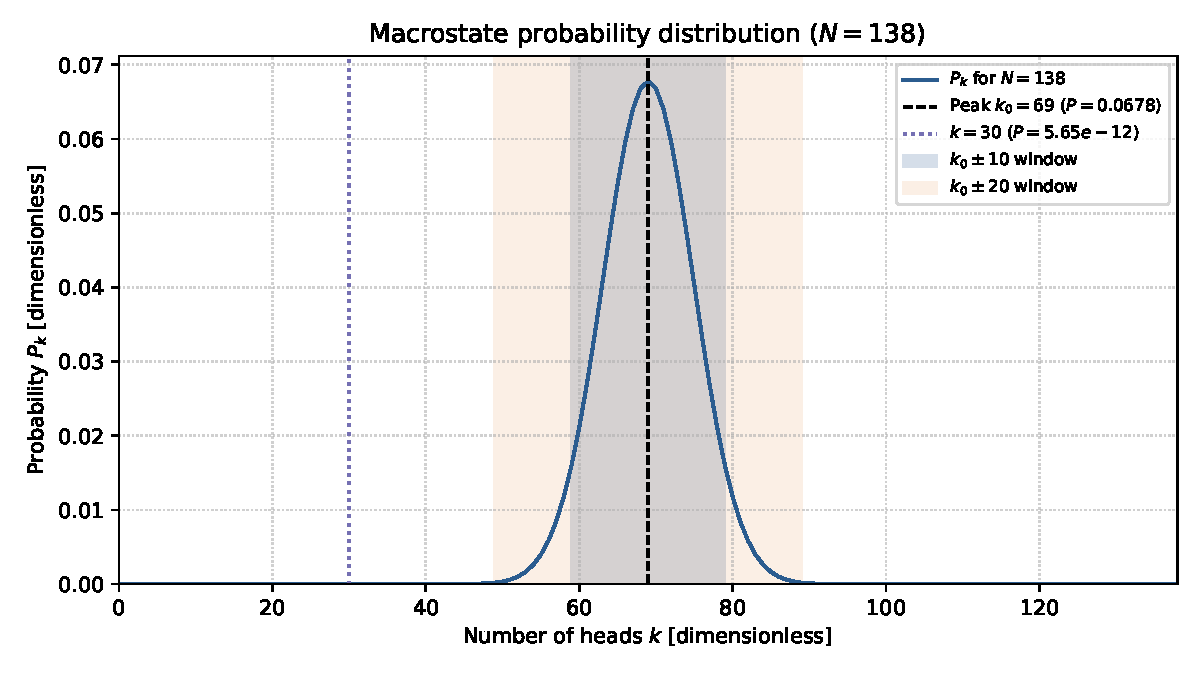
\includegraphics[width=0.78\textwidth]{figures/figure_probabilities}
\caption{Macrostate probability $P_k$ for $N=138$ coins (dimensionless). Dashed: most probable macrostate
$k_0=69$; shaded: $k_0\pm10$ (dark) and $k_0\pm20$ (light) windows; dotted: $k=30$.}
\label{fig:prob}
\end{figure}
The macrostate with 30 heads is $P_{69}/P_{30}=1.2\times10^{10}$ times less probable than the peak, only because it has fewer
microstates ($\Om=1.97\times10^{30}$ versus $2.36\times10^{40}$); each microstate has the same probability $2^{-138}$.
The peak holds only $6.8\%$ of the probability, but the $\pm10$ window ($1.7\sigma$, $\sigma=5.87$) holds $92.7\%$ and the $\pm20$ window
($3.4\sigma$) $99.96\%$, in agreement with the Gaussian \eqref{eq:gauss} ($0.9262$, $0.99952$).

\subsection{Entropy changes}
We compute $\Delta S_{k_1k_2}\equiv S(k_1)-S(k_2)$, so that $\Delta S/\kB=\ln[\Om(N,k_1)/\Om(N,k_2)]$, with $\kB=1.380649\times10^{-23}$~J/K (exact SI value); results are in Table~\ref{tab:entropy}.
\begin{table}[H]
\centering\small
\begin{tabular}{@{}cclrrr@{}}
\toprule
item & $(k_1,k_2)$ & states & $\Delta S/\kB$ & $\Delta S$ (J/K) & $\Om_1/\Om_2$ \\ \midrule
e) & $(94,69)$ & high disorder $\to$ maximum & $-9.1974$ & $-1.270\times10^{-22}$ & $1.013\times10^{-4}$ \\
f) & $(79,69)$ & moderate $\to$ maximum & $-1.4438$ & $-1.993\times10^{-23}$ & $0.2360$ \\
g) & $(69,20)$ & maximum $\to$ high order & $+38.2003$ & $+5.274\times10^{-22}$ & $3.892\times10^{16}$ \\ \bottomrule
\end{tabular}
\caption{Entropy differences for $N=138$ (numerical uncertainty $<10^{-13}$ in $\Delta S/\kB$).}
\label{tab:entropy}
\end{table}
Table~\ref{tab:entropy} shows that the maximum entropy is at $k=N/2$: moving away from it reduces $S$. In cases e) and f), $S(k_1)<S(k_2)$ and hence
$\Delta S<0$. In case g), $S(k_1)>S(k_2)$ and $\Delta S>0$, with a much larger magnitude because $k=20$ is far from the peak
($\Om_1/\Om_2\sim10^{16}$).

\subsection{Thermodynamic implications}\label{sec:thermo}
\textbf{h) Time to a highly ordered state.} We assume a tossing rate of $N$ coins per second, i.e.\ one independent trial of the whole system per second, and the probability of success is
$P_8=\Om(138,8)/2^{138}=7.61\times10^{-30}$. The number of trials until the first success is geometric with mean
\begin{equation}
  \langle t\rangle=\frac1{P_8}=1.31\times10^{29}\ \mathrm s=4.2\times10^{21}\ \mathrm{yr}\approx3\times10^{11}\ \text{ages of the universe}
\end{equation}

\textbf{i) Likelihood ratio.} The ratio between the most probable macrostate and another one is
\begin{equation}
\frac{P_{k_a}}{P_{k_b}}=\frac{\Om(N,k_a)}{\Om(N,k_b)}=e^{\Delta S_{k_ak_b}/\kB}.
\end{equation}
For $M\pm10$ heads ($k=48$ and $k=28$, with $M=38$) the ratios are $629.8$ and $1.65\times10^{11}$, respectively.

\textbf{j) Second Law.} None of the obtained results contradicts the Second Law. Statistically, an isolated system evolves towards macrostates of larger multiplicity
because they are more probable, not because decreases of $S$ are forbidden. The transitions obtained for the analysed entropy changes are improbable but possible.
An example is case g), where the likelihood ratio of the move from the maximum to $k=20$ is $e^{-38.2}=2.6\times10^{-17}$, which shows that it is very unlikely to be observed.
In contrast, for case f) $\Delta S/\kB=-1.4$, which corresponds to visible fluctuations.
This way, it can be reaffirmed that the Second Law of Thermodynamics holds for these cases.

\subsection{Large-$N$ limit ($N\to10^{23}$)}\label{sec:largeN}
All items are re-evaluated for $N=10^{23}$ with the Gaussian form \eqref{eq:gauss}, and with $\ln\binom Nk=\sum_{j=0}^{k-1}\ln[(N-j)/(k-j)]$ for small $k$ (items a and h). The results are in Table~\ref{tab:large}.
\begin{table}[H]
\centering\small
\begin{tabular}{@{}ll@{}}
\toprule
item & result for $N=10^{23}$ ($\sigma=1.58\times10^{11}$) \\ \midrule
a) $P_{30}$ & $\log_{10}P_{30}=-3.01\times10^{22}$ (zero in practice) \\
b) $P_{N/2}$ & $2.52\times10^{-12}$ \\
c), d) $\Delta P$, $N/2\pm10$, $\pm20$ & $5.30\times10^{-11}$, $1.03\times10^{-10}$ \\
e), f) $\Delta S/\kB$ & $-1.25\times10^{-20}$, $-2.0\times10^{-21}$ \\
g) $\Delta S$ & $6.93\times10^{22}\,\kB\simeq N\kB\ln2=0.957$~J/K \\
h) waiting time & $\log_{10}t=3.01\times10^{22}$ ($t$ in s) \\
i) likelihood ratio & $P_{N/2}/P_{N/2\pm10}-1=2.0\times10^{-21}$ \\ \bottomrule
\end{tabular}
\caption{Items a--i for $N=10^{23}$ (analytic; relative error of $\ln\Om$ is $O(1/N)$).}
\label{tab:large}
\end{table}
Entropy differences between nearby macrostates vanish, whereas the difference to an ordered
state is extensive, $\simeq N\kB\ln2\approx0.96$~J/K, and the waiting time is $10^{3\times10^{22}}$~s. As a result, the Second Law becomes deterministic for $N\to\infty$, since the relative fluctuations scale as $N^{-1/2}\to0$.

\section{Conclusions}
The results obtained for the system of coins agree with the statistical picture described in the manual. In the enumeration of microstates, storing every state is limited by memory ($N=27$ was the last size completed, and $N=28$ exhausted the RAM), whereas the generator only keeps one counter per macrostate, so its cost is dominated by time, which grows by $2^N$ and gives the extrapolated limit $N_{\max}\approx31$ for five minutes.
For the multiplicities, exact integers reached $N=354,419$ in the calculation but only $N=1028$ in the plot, because of the double-precision overflow; computing in log-space removes this limit, and the practical maximum, set by memory and rounding, is $N\sim10^7$.

For the team size $N=138$, the distribution is symmetric and peaked at $k=N/2=69$ ($P_{69}=0.0678$), and the probability is concentrated around it: $92.7\%$ lies within $\pm10$ heads and $99.96\%$ within $\pm20$, in agreement with the Gaussian approximation. States far from the peak, such as $k=30$, are less probable only because they have fewer microstates, since every microstate has the same probability $2^{-138}$.
The entropy is maximal at $k=N/2$, and the ordered macrostate with 20 heads has $38.2\,\kB$ less entropy. Reaching a state of 8 heads by random tossing would take $\sim4\times10^{21}$ years, so such low-entropy states are not forbidden but extremely improbable, and the Second Law is not contradicted by any of the results.
For $N\sim10^{23}$ the relative width of the distribution is $N^{-1/2}=3.2\times10^{-12}$ and the entropy gap to an ordered state is extensive, $\simeq N\kB\ln2\approx0.96$~J/K, so the macroscopic state is sharply defined and the Second Law becomes deterministic.

\appendix
\section{All microstates for $N=7$}\label{app:n7}
All $2^7=128$ microstates are listed in Table~\ref{tab:n7full}, grouped by number of heads $k$, as in Table~1 of the lab manual.

\begin{table}[H]
\centering\small
\begin{tabular}{@{}ccrp{10.2cm}@{}}
\toprule
heads $k$ & tails $7-k$ & $\Om(7,k)$ & microstates \\ \midrule
7 & 0 & 1 & {\raggedright\ttfamily\scriptsize HHHHHHH\par} \\
\midrule
6 & 1 & 7 & {\raggedright\ttfamily\scriptsize THHHHHH HTHHHHH HHTHHHH HHHTHHH HHHHTHH HHHHHTH HHHHHHT\par} \\
\midrule
5 & 2 & 21 & {\raggedright\ttfamily\scriptsize TTHHHHH THTHHHH THHTHHH THHHTHH THHHHTH THHHHHT HTTHHHH HTHTHHH HTHHTHH HTHHHTH HTHHHHT HHTTHHH HHTHTHH HHTHHTH HHTHHHT HHHTTHH HHHTHTH HHHTHHT HHHHTTH HHHHTHT HHHHHTT\par} \\
\midrule
4 & 3 & 35 & {\raggedright\ttfamily\scriptsize TTTHHHH TTHTHHH TTHHTHH TTHHHTH TTHHHHT THTTHHH THTHTHH THTHHTH THTHHHT THHTTHH THHTHTH THHTHHT THHHTTH THHHTHT THHHHTT HTTTHHH HTTHTHH HTTHHTH HTTHHHT HTHTTHH HTHTHTH HTHTHHT HTHHTTH HTHHTHT HTHHHTT HHTTTHH HHTTHTH HHTTHHT HHTHTTH HHTHTHT HHTHHTT HHHTTTH HHHTTHT HHHTHTT HHHHTTT\par} \\
\midrule
3 & 4 & 35 & {\raggedright\ttfamily\scriptsize TTTTHHH TTTHTHH TTTHHTH TTTHHHT TTHTTHH TTHTHTH TTHTHHT TTHHTTH TTHHTHT TTHHHTT THTTTHH THTTHTH THTTHHT THTHTTH THTHTHT THTHHTT THHTTTH THHTTHT THHTHTT THHHTTT HTTTTHH HTTTHTH HTTTHHT HTTHTTH HTTHTHT HTTHHTT HTHTTTH HTHTTHT HTHTHTT HTHHTTT HHTTTTH HHTTTHT HHTTHTT HHTHTTT HHHTTTT\par} \\
\midrule
2 & 5 & 21 & {\raggedright\ttfamily\scriptsize TTTTTHH TTTTHTH TTTTHHT TTTHTTH TTTHTHT TTTHHTT TTHTTTH TTHTTHT TTHTHTT TTHHTTT THTTTTH THTTTHT THTTHTT THTHTTT THHTTTT HTTTTTH HTTTTHT HTTTHTT HTTHTTT HTHTTTT HHTTTTT\par} \\
\midrule
1 & 6 & 7 & {\raggedright\ttfamily\scriptsize TTTTTTH TTTTTHT TTTTHTT TTTHTTT TTHTTTT THTTTTT HTTTTTT\par} \\
\midrule
0 & 7 & 1 & {\raggedright\ttfamily\scriptsize TTTTTTT\par} \\

\bottomrule
\end{tabular}
\caption{All $2^7=128$ microstates of $N=7$ coins, one row per macrostate (H = heads, T = tails); $\Om(7,k)$ is the number of microstates in each row and the rows add up to $128$.}
\label{tab:n7full}
\end{table}
\section{AI collaboration statement}
AI assistants (Claude, Gemini and Copilot) were used for drafting code, code redefinition and proper implementation of mathematical procedures and contraints. Additionally, the AI assistant were applied for the elaboration of some comments and to look for Git Hub implementation commands. Every prompt, generated code and modification is logged in \texttt{AI\_STATEMENT.md}.
All AI-generated logic is covered by tests of each section and was it reviewed by the corresponding team member who implemented it.
\section{Github link}
In this section, the link to the Github was inserted: https://github.com/100542175/LAB-1-STATISTICAL-PHYSICS
\end{document}
